\documentclass{beamer}
\usetheme{metropolis}

\usepackage{amsmath, amssymb, amsthm}
\usepackage{cite, graphicx, latexcolors}
\usepackage{ragged2e, microtype}
\usepackage{url, parskip, hyperref}
\usepackage{array, tikz, flowchart}
\usepackage[dvipsnames]{xcolor}
\usepackage{media9}
\usepackage{caption}

\hypersetup{colorlinks=true,}
\setbeamercolor{title}{fg=orange}

\usetikzlibrary{arrows.meta, calc, chains, quotes, positioning, shapes.geometric}
\tikzset{FlowChart/.style={
    node distance = 5mm and 10mm,
    start chain = A going right,
    base/.style = {draw, minimum width=16mm, minimum height=19mm, align=center, on chain=A, text width=4cm},
    process/.style = {base},
    rounded/.style = {base, rounded corners},
    every edge quotes/.style = {auto=right}
}}

\newcommand{\videofolder}{videos/}
\title[NMPC Implementation]{
    \textbf{Implementation of Nonlinear MPC on a \\
                Quadreped robot}
}
\subtitle[Presentation]{\textcolor{brown}{
    \textbf{FoR Project Presentation - 4} \\
}}
\author[BRAMA]{%
Team-5 BRAMA \quad \scriptsize \\
\begin{tabular}{lllll}
    Biswadeep &
    Rithwik &
    Akhil &
    Moin &
    Ashrith
\end{tabular}
\vspace{2em}
}
\institute[IISc]{    
    Robert Bosch Centre for Cyber Physical Systems,\\
    Indian Institute of Science
}
\date{\scriptsize\today}
\begin{figure}
    
\includegraphics[width=0.25\linewidth]{Common/rbccps.png}
\end{figure}


\begin{document}

% \section*{Titlepage}
\begin{frame}\titlepage\end{frame}\normalfont


% \section*{Outline}
\begin{frame}{Outline}
	\begin{enumerate}
            \item Introduction
		\item Overview of the paper
            \item Methodology (from paper)
            \item Implementation Approach
            \item Demonstrations
            \item Technical Difficulties
            \item Learnings
            \item Potential Developments
            \item References
	\end{enumerate}
\end{frame}\normalfont

\begin{frame}{Introduction}
\begin{itemize}
  \item Achieving animal-like mobility in robots requires controlling dynamics while managing hardware limitations and the environment interactions.
  \item MPC, popular due to advances in computing and optimization, enables real-time execution on embedded systems with system dynamics and constraints.
  \item Direct MPC on high DoF systems requires heavy computation, limiting its use on embedded platforms, so simplified models are used to balance complexity and essential dynamics.
\end{itemize}

\end{frame}\normalfont

\begin{frame}{Introduction}
\begin{itemize}
  \item Euler angles representation has the singularity issue (Gimbal lock)
  \item Quaternion ambiguity could cause unwinding phenomenon
  \item The rotation matrix possesses advantages as a global parametrization that is compact and singularity-free 
\end{itemize}

\end{frame}\normalfont

\begin{frame}{Overview of the paper}
\begin{itemize}
  \item Introduce a novel MPC formulation for controlling legged robots in dynamic 3D motions using \textbf{rotation matrices}
  \item A novel vectorization technique along with a deliberately chosen cost function enables the transcription of RF-MPC into a \textbf{Quadratic Program (QP)}
  \item Implement the Representation free -MPC on a quadruped. 
\end{itemize}

\end{frame}\normalfont

\begin{frame}{Methodology (from paper)}
    \begin{itemize}
        \item Simplify the robot to a single rigid-body (SRB) model centered at the center of mass, with ground reaction forces as inputs.
        \item Linearize system dynamics and discretize equations
        \item Formulate MPC using a quadratic cost function.
        \item Incorporate physical constraints into MPC for real-time optimization of stable and efficient motion planning.
    \end{itemize}
    \vfill % This will add vertical space to push the image down to the bottom
    
\end{frame}\normalfont

\begin{frame}{RBD model}


\begin{figure}
    \centering
    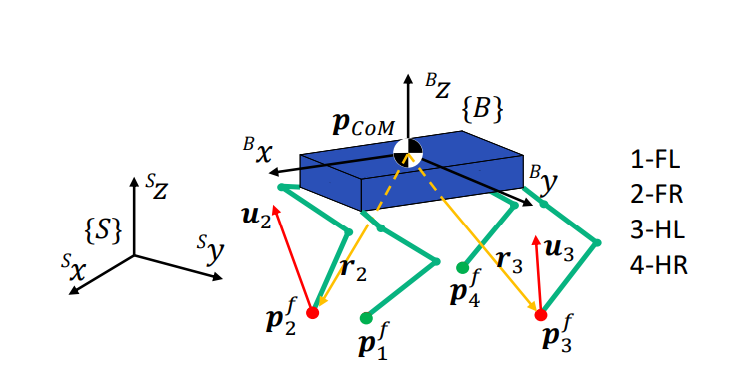
\includegraphics[width=0.5\linewidth]{Presentation-4/images/Illustration-RBD-model.png}
    \caption{Illustration of the 3D Single RBD model}
    \label{fig:rbd-model}
\end{figure}

\begin{equation*}
    \mathbf{\dot{x}} = f(\mathbf{x}, \mathbf{u}) = 
    \begin{bmatrix}
    \mathbf{\dot{p}} \\
    \mathbf{\ddot{p}} \\
    \mathbf{\dot{R}} \\
    {}^{B}\boldsymbol{\dot{\omega}}
    \end{bmatrix}
    =
    \begin{bmatrix}
    \mathbf{\dot{p}} \\
    \frac{1}{M} \mathbf{f} - \mathbf{a_g} \\
    \mathbf{R} \cdot {}^{B}\hat{\boldsymbol{\omega}} \\
    {}^{B} \mathbf{I}^{-1}(R^T \boldsymbol{\tau} - {}^{B}\hat{\boldsymbol{\omega}} {}^{B} \mathbf{I} {}^{B}\boldsymbol{\omega})
    \end{bmatrix}
\end{equation*}

\begin{itemize}
    \scriptsize
    \item $\mathbf{R}$ is the rotation matrix of the body frame $\{ \mathbf{B} \}$ expressed in the inertial frame $\{ \mathbf{S} \}$
    \item ${}^{B} \mathbf{I} \in \mathbb{R}^{3\times 3}$ is the fixed moment of inertia tensor in the body frame $\{ \mathbf{B} \}$
\end{itemize}
\end{frame}


\begin{frame}{Non-Linear MPC formulation}
\begin{equation*}
\begin{aligned}
    & \text{minimize} \quad \sum_{k=1}^{N-1} \ell(\mathbf{x_k}, \mathbf{u_k}) + \ell_T(\mathbf{x_N}) \\
    & \text{subject to} \quad \mathbf{x_{k+1}} = g(\mathbf{x_k}, \mathbf{u_k}), \quad \mathbf{x_1} = \mathbf{x_\text{op}}, \\
    & \mathbf{x_k} \in \mathbb{X}, \quad k = 1, 2, \dots, N, \\
    & \mathbf{u_k} \in \mathbb{U}, \quad k = 1, 2, \dots, N-1
\end{aligned}
\end{equation*}
\begin{itemize}
    \item Stage cost: $ \ell(\mathbf{x_k}, \mathbf{u_k}) = \lVert \mathbf{x_k} - \mathbf{x_{d, k}} \rVert ^ 2 \mathbf{Q_x} + \lVert \mathbf{u_k} - \mathbf{u_{d, k}} \rVert ^ 2 \mathbf{R_u}$
    \item Terminal cost: $ \ell_T $
    \item Error terms $\leftrightarrow$ Quadratic forms
    \item Force Constraints
\end{itemize}
\end{frame}

\begin{frame}{Variation-based Linearisation}
\begin{block}{Rotation Matrix Approximation on \(\text{SO}(3)\)}
\item Assumption: Predicted variables are close to the
operating point
\[
R_k \approx R_\text{op} \exp(\delta R_k) \approx R_\text{op}(I + \delta R_k)
\]
\implies
\dot{\mathbf{R_k}} & \approx \mathbf{R_{op}}\mathbf{\hat \omega_{op}} + \mathbf{R_{op}}\mathbf{\hat\omega_{op}}\mathbf{\delta R_k} + \mathbf{R_{op}}\widehat{\delta\mathbf{\omega_k}}


\item The Dynamics of \(\dot{\omega}_k\) is linearized as
\[
    ^B I \dot{\omega}_k = R_{op}^T \tau_{op} + \delta R_k^T \tau_{op} + R_{op}^T \delta \tau_k - \hat{\omega}_{op} {}^B I \omega_{op} - \delta \hat{\omega}_k {}^B I \omega_{op} - \hat{\omega}_{op} {}^B I \delta \omega_k
\]
\end{block}

\item Vectorization method using the Kronecker products is used to optimize matrix-matrix computations
\begin{align*}
\text{vec}(R_{op} \hat{\omega}_{op} \delta R_k) &= (I \otimes R_{op} \hat{\omega}_{op}) N \xi_k \\
\text{vec}(R_{op} \widehat{\delta \omega_k}) &= (I \otimes R_{op}) \text{vec}(\delta d \omega_k)
\end{align*}

\end{frame}

\begin{frame}{Implementation Approach}
\begin{itemize}
    \item Two controllers: \texttt{StanceController} and \texttt{SwingController}
    \item Time for one gait cycle was set to \texttt{400 ms}, with 50\% swing time and 50\% stance time
    \item Gait modes: Stand, March, Trot
\end{itemize}
\begin{center}
        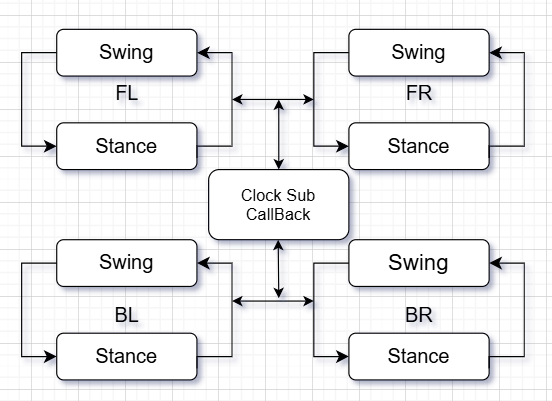
\includegraphics[width=0.4\textwidth]{Presentation-4/images/clock_sub_callback.png}
        \captionof{figure}{Switching Controllers}
\end{center}
\end{frame}\normalfont

\begin{frame}{Implementation Approach}
Callbacks
\begin{itemize}
    \item \texttt{clock\_sub\_callback}
    \begin{itemize}
        \item Periodically check gait mode and configure leg states accordingly
    \end{itemize}
    
    \item \texttt{timer\_pub\_callback}
    \begin{itemize}
        \item Get torques from controllers and publish to joints
    \end{itemize}

    \item \texttt{teleop\_sub\_callback}
    \begin{itemize}
        \item Publish \texttt{teleop} commands to the bot to apply twists for movement
    \end{itemize}
\end{itemize}
\end{frame}\normalfont

\begin{frame}{Implementation Approach}
\texttt{StanceController}
\begin{itemize}
    \item Runs MPC to make the bot to stand upright, by calculating the desired ground reaction forces

    \item \texttt{linearise()}
    \begin{itemize}
        \item Successive variation-based linearisation
    \end{itemize}

    \item \texttt{vectorise()}
        \begin{itemize}
        \item Kronecker products and vectorisation
    \end{itemize}

    \item \texttt{solveMPC()}
    \begin{itemize}
        \item Compute optimisation parameters and solve it
        \item Solver used: \texttt{qpSWIFT}
    \end{itemize}
\end{itemize}
\end{frame}\normalfont

\begin{frame}{Implementation Approach}
\texttt{SwingController}
\begin{itemize}
    \item PD control based; Different parameters tuned for each leg
    \item The legs in swing are moved by calculating foot positions using an elliptical curve
    \item Parameters:
    \begin{itemize}
        \item \texttt{swing\_time}: Time spent in one swing cycle; \\
        Set to 50\% of \texttt{gait\_time}, i.e., \texttt{200 ms}
        \item \texttt{z\_max}: Maximum height each foot should raise while moving
    \end{itemize}
\end{itemize}
\end{frame}\normalfont

\begin{frame}{Implementation Approach}
\texttt{SwingController}
\begin{figure}
    \centering
    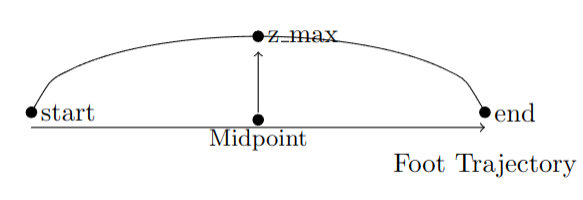
\includegraphics[width=0.75\linewidth]{Presentation-4/images/ellipse.png}
    \caption{Ellipse}
\end{figure}
\end{frame}\normalfont

\begin{frame}{Implementation Approach}
Gait modes
\begin{itemize}
    \item Stand
    \begin{itemize}
        \item Just \texttt{StanceController} with all legs in stance
        \item Default while starting before other gaits are tried out
    \end{itemize}

    \item March
    \begin{itemize}
        \item Alternate legs set in stance and swing
    \end{itemize}

    \item Trot
    \begin{itemize}
        \item Similar to march, with translational movement done through \texttt{teleop}
    \end{itemize}
\end{itemize}
\end{frame}\normalfont

\begin{frame}{RQT GRAPH}
\begin{figure}
    \centering
    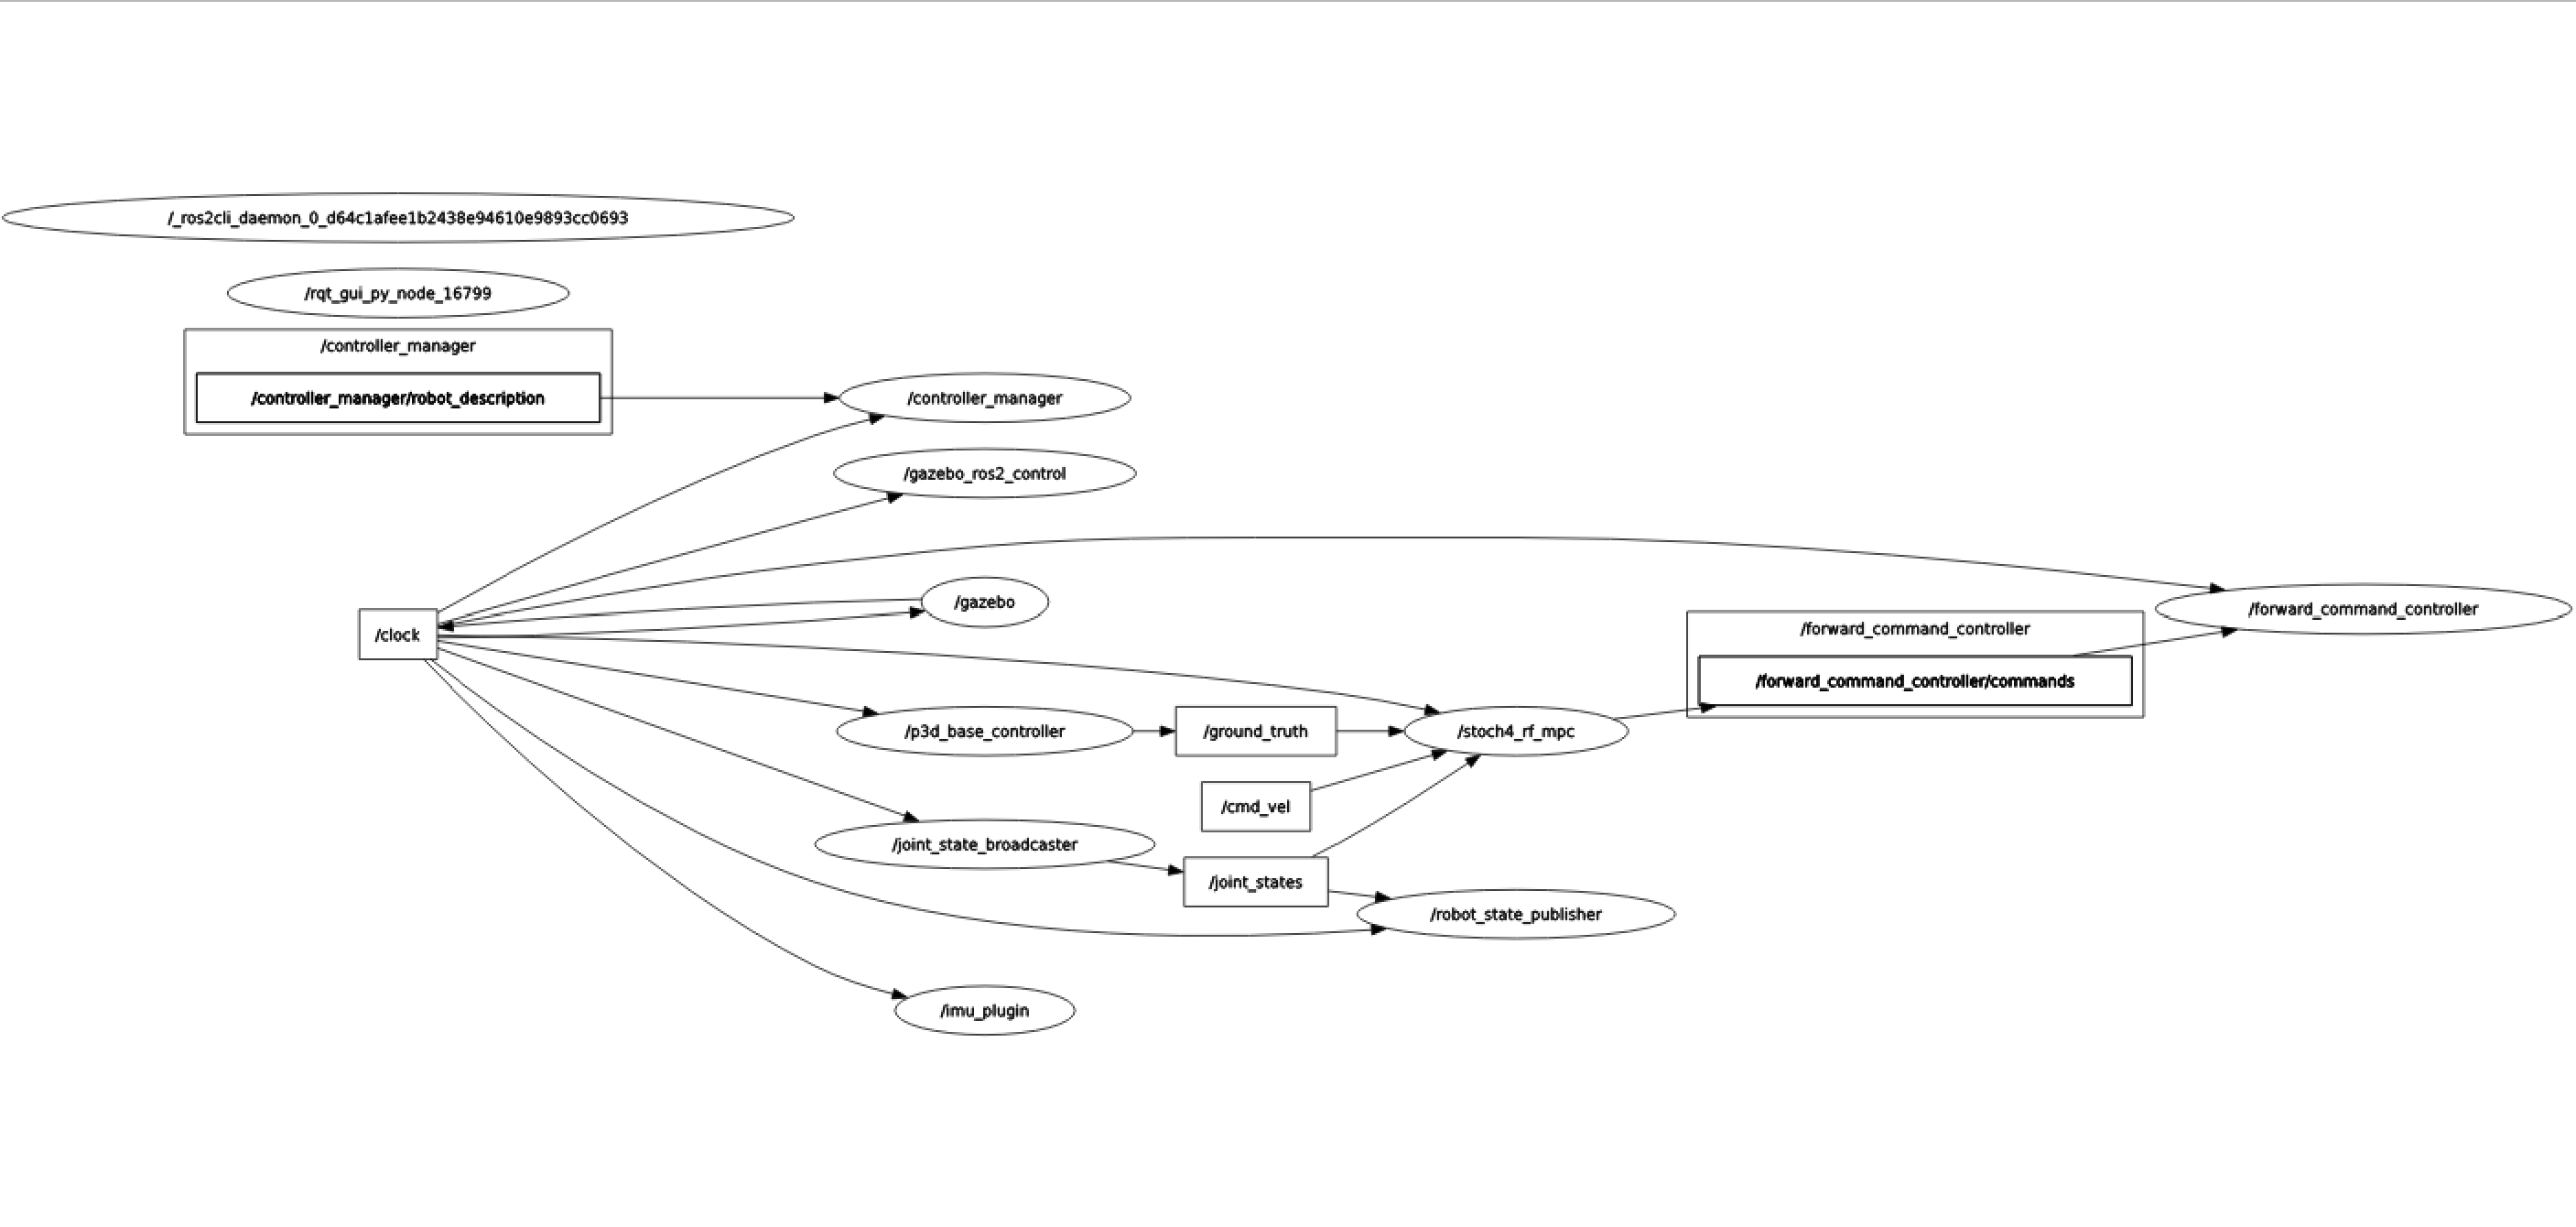
\includegraphics[width=1.0\linewidth]{Presentation-4/images/rqt-graph.png}
    \caption{Nodes and Topics}
    \label{fig:enter-label}
\end{figure}
\end{frame}\normalfont

\begin{frame}{Demonstrations}
    \begin{itemize}
        \item \href{\videofolder long-march.webm}{long-march}
        \item \href{\videofolder low-ground.mp4}{low-ground}
        \item \href{\videofolder trot-forward-backward.mp4}{trot-forward-backward}
    \end{itemize}
    \vspace*{2em}
    GitHub Repo: \url{https://github.com/AshrithSagar/Stoch4-MPC}
\end{frame}\normalfont

\begin{frame}{Technical Difficulties}
\begin{itemize}
    \item Misaligned collision models led to unexpected ground interaction behaviors.
    \item Challenges in tuning MPC parameters caused oscillations and sluggish responses.
    \item High computational demands caused lags and crashes.
    \item Flying Off: Gazebo spawn entity causing the robot to fly off
    \item Falling Down: Control manager was not loading in time
    \item Slipping: Incorrect foot placement and friction coefficient
    \item Z-Axis Stability Problem: Flying off after any keyboard press
    \item Latency in ROS affecting the coordination between controllers and state estimators.
\end{itemize}
\end{frame}\normalfont

\begin{frame}{Learnings}
\begin{itemize}
    \item Gained experience working with ROS and Gazebo for simulation and control.
    \item Overcame challenges in legged locomotion, focusing on stability and adaptability.
    \item Explored different movement patterns in quadrupeds, enhancing mobility.
    \item Developed and integrated StanceController and SwingController for real-time gait and posture control.
    \item Used rotation matrices to overcome gimbal lock and unwinding in robot orientation.
    \item Implemented various gait patterns, including standing, marching, and trotting, for quadruped robots.
\end{itemize}
\end{frame}\normalfont

\begin{frame}{Potential Developments}
\begin{itemize}
    \item Autonomous walking with accurate foot positioning for stability.
    \item Balances weight on remaining legs for stable motion.
    \item Capable of walking uphill and downhill slopes.
    \item Recovers from disturbances during motion.
    \item Smooth, coordinated limb movements for efficiency.
    \item Maintains posture and avoids falling on uneven surfaces.
\end{itemize}
\end{frame}\normalfont


\begin{frame}{References}

\begin{itemize}
  \item Y. Ding, A. Pandala, C. Li, Y. -H. Shin and H. -W. Park, "Representation-Free Model Predictive Control for Dynamic Motions in Quadrupeds," in IEEE Transactions on Robotics, vol. 37, no. 4, pp. 1154-1171, Aug. 2021, doi: 10.1109/TRO.2020.3046415.

  \item Yanran Ding, Abhishek Pandala, and Hae-Won Park. 2019. Real-time Model Predictive Control for Versatile Dynamic Motions in Quadrupedal Robots. In 2019 International Conference on Robotics and Automation (ICRA). IEEE Press, 8484–8490. https://doi.org/10.1109/ICRA.2019.8793669


  \item \href{https://github.com/erwincoumans/motion_imitation/tree/master/mpc_controller}{github : erwincoumans/motion\_imitation}

  \item \href{https://github.com/YanranDing/RF-MPC}{github : YanranDing/RF-MPC}

  
\end{itemize}

\end{frame}\normalfont
    
\begin{frame}
	\LARGE{Thank You!}
\end{frame}\normalfont

\end{document}
